\SbSSCT{Dans le texte}{In the text}


%\subsubsection{Sans option de décalage}
\SbSbSSCT{Sans option de décalage}{Without offset}

\begin{center}
\RRR{12-2}
\end{center}

\TFRGB{dessin directement  dans le texte}{picture in the text}  \tikz \draw[blue] (0,0) rectangle(2,2); \tikz \draw[blue] (0,0) circle (1);\TFRGB{ici est inclus le code suivant}{here is the following code} : \BS{tikz} \BS{draw} (0,0) rectangle(2,2);\BS{tikz} \BS{draw} (0,0) circle (1);
\bigskip

%\subsubsection{Avec décalage nul}
\SbSbSSCT{Avec décalage nul}{With zero offset}

\TFRGB{dessin directement  dans le texte}{picture in the text}  \tikz[baseline=0pt] \draw[blue] (0,0) rectangle(2,2); \tikz[baseline=0pt] \draw[blue] (0,0) circle (1);\TFRGB{ici est inclus le code suivant}{here is the following code} : \BS{tikz}[\RDD{baseline}=0pt] \BS{draw} (0,0) rectangle(2,2);\BS{tikz}[\RDD{baseline}=0pt] \BS{draw} (0,0) circle (1);
\bigskip


\bigskip

%\subsubsection{Avec décalage }
\SbSbSSCT{Avec décalage}{With an offset}

\TFRGB{dessin directement  dans le texte}{picture in the text}  \tikz[baseline=1cm] \draw[blue] (0,0) rectangle(2,2); \tikz[baseline=1cm] \draw[blue] (0,0) circle (1);\TFRGB{ici est inclus le code suivant}{here is the following code} : \BS{tikz}[\RDD{baseline}=1cm] \BS{draw} (0,0) rectangle(2,2);\BS{tikz}[\RDD{baseline}=1cm] \BS{draw} (0,0) circle (1);


\newpage
%----------------------------------------------------------
\SbSSCT{Dans un environnement tikzpicture}{In a tikzpicture environment}

\begin{center}
\RRR{12-1}
\end{center}

\begin{tabular}{|l|l|} \hline  
 
\TFRGB{texte avant}{text before} 
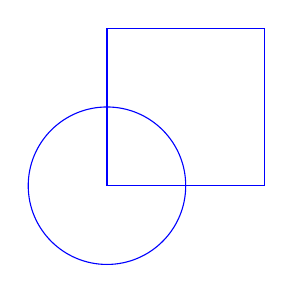
\begin{tikzpicture}[blue]
\draw (0,0) rectangle(2,2); 
 \draw (0,0) circle (1);
\end{tikzpicture}
\TFRGB{texte après}{text after} 
&  
\parbox[b]{8cm}{
\TFRGB{texte avant}{text before} \\
\ESS{begin\AC{tikzpicture}}[blue] \\
\BS{draw} (0,0) rectangle(2,2);  \\
\BS{draw} (0,0) circle (1); \\
\ESS{end\AC{tikzpicture}}\\
\TFRGB{texte après}{text after} \\
}
\\ \hline 
\end{tabular} 

\bigskip


\begin{tabular}{|l|l|} \hline 
\TFRGB{texte avant}{text before} 
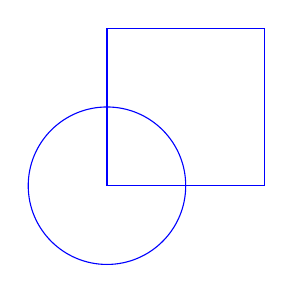
\begin{tikzpicture}[blue,baseline=0pt]
\draw (0,0) rectangle(2,2); 
 \draw (0,0) circle (1);
\end{tikzpicture}
\TFRGB{texte après}{text after} 
&  
\parbox[c]{8cm}{
\TFRGB{texte avant}{text before} \\
\BS{begin}\AC{tikzpicture}[blue,\RDD{baseline}=0pt] \\
\BS{draw} (0,0) rectangle(2,2);  \\
\BS{draw} (0,0) circle (1); \\
\BS{end}\AC{tikzpicture} \\
\TFRGB{texte après}{text after} \\
}
\\ \hline 
\end{tabular} 

\bigskip
\noindent

\begin{tabular}{|l|l|} \hline 
\TFRGB{texte avant}{text before} 
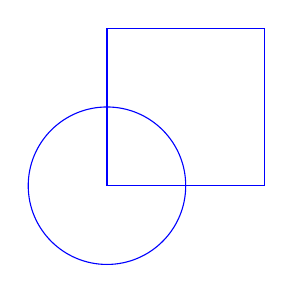
\begin{tikzpicture}[blue,baseline=1cm]
\draw (0,0) rectangle(2,2); 
 \draw (0,0) circle (1);
\end{tikzpicture}
\TFRGB{texte après}{text after} 
&  
\parbox[t]{8cm}{
\TFRGB{texte avant}{text before} \\
\BS{begin}\AC{tikzpicture}[blue,\RDD{baseline}=1cm] \\
\BS{draw} (0,0) rectangle(2,2);  \\
\BS{draw} (0,0) circle (1); \\
\BS{end}\AC{tikzpicture} \\
\TFRGB{texte après}{text after} \\
}
\\ \hline 
\end{tabular} 




%\subsection{Dans un environnement fbox}
\SbSSCT{Dans un environnement fbox}{In a fbox environment}

\noindent

\begin{tabular}{|l|l|} \hline 
\TFRGB{texte avant}{text before}
\fbox{ 
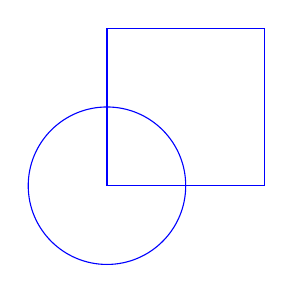
\begin{tikzpicture}[blue,baseline=0pt]

\draw (0,0) rectangle(2,2); 
 \draw (0,0) circle (1);
\end{tikzpicture}}
\TFRGB{texte après}{text after} 
&  
\parbox[c]{8cm}{
\TFRGB{texte avant}{text before}\\
\BSS{fbox}\{ \\ 
\BS{begin}\AC{tikzpicture}[blue,\RDD{baseline}=0pt] \\
\BS{draw} (0,0) rectangle(2,2);  \\
\BS{draw} (0,0) circle (1); \\
\BS{end}\AC{tikzpicture} \\
 \}\\
\TFRGB{texte après}{text after} \\
}
\\ \hline 
\end{tabular}

%\subsection{Modification du cadrage}
\SbSSCT{Modification du cadrage}{Bounding box}

\begin{center}
\RRR{15-8}
\end{center}

\bigskip

\begin{tabular}{|c|c|}  \hline  
\multicolumn{2}{|l|}{\BS{draw} [\RDD{use as bounding box}] (1,0) rectangle (2,1);}\\ 
\multicolumn{2}{|l|}{\BS{draw}[blue] (-1,0) - - (3,1);} \\\hline 
texte avant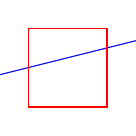
\begin{tikzpicture}
\draw [use as bounding box] (1,0) rectangle (2,1);
\draw[blue] (-1,0) - - (3,1);
\draw [red](1,0) rectangle (2,1);
\end{tikzpicture}texte après
&
texte avant 

\begin{tikzpicture}
\draw [use as bounding box] (0,0) rectangle (0,0);
\draw[blue] (-1,0) - - (3,1);
\draw [red](0,0) rectangle (0,0);
\end{tikzpicture}
texte après  
\\ \hline 
(1,0) rectangle (2,1) & (0,0) rectangle (0,0)
\\ \hline 
\end{tabular} 

\bigskip

\begin{tabular}{|c|c|} \hline
\multicolumn{2}{|l|}{texte avant. \BS{begin\AC{tikzpicture}} [\RDD{trim left}=1cm] }\\ 
\multicolumn{2}{|l|}{\BS{draw}[blue] (-1,0) - - (3,1); \BS{draw}[red] (0,0) grid (2,1);} \\
\multicolumn{2}{|l|}{ \BS{end\AC{tikzpicture}}texte après }\\ 
\hline 
  
texte avant.%
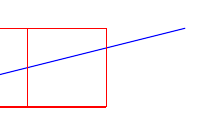
\begin{tikzpicture}[trim left=1cm]
\draw[blue] (-1,0) - - (3,1);
\draw [red](0,0) grid (2,1);
\end{tikzpicture}%
texte après
&  
texte avant.%
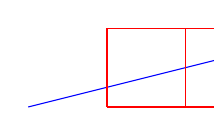
\begin{tikzpicture}[trim right= 1cm]
\draw[blue] (-1,0) - - (3,1);
\draw [red](0,0) grid(2,1);
\end{tikzpicture}%
texte après
\\ \hline  
[\RDD{trim left}=1cm]
&  
[\RDD{trim right}= 1cm]
\\ \hline 
\end{tabular} 

%\SbSSCT{Tracer les limites du dessin}{Drawing the bounding box}

 

\bigskip

\begin{tabular}{|l|l|} \hline  
\TFRGB{texte avant}{text before} 
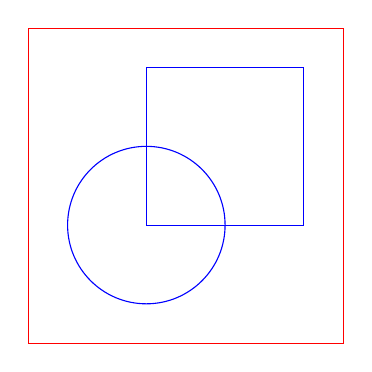
\begin{tikzpicture}[blue]
\draw [red,use as bounding box] (-1.5,-1.5) rectangle (2.5,2.5);
\draw (0,0) rectangle(2,2); 
 \draw (0,0) circle (1);
\end{tikzpicture}
\TFRGB{texte après}{text after} 
&  
\parbox[b]{10cm}{
\TFRGB{texte avant}{text before} \\
\ESS{begin\AC{tikzpicture}}[blue] \\
\BS{draw} [red,\RDD{use as bounding box}] (-1.5,-1.5) rectangle (2.5,2.5); \\
\BS{draw} (0,0) rectangle(2,2);  \\
\BS{draw} (0,0) circle (1); \\
\ESS{end\AC{tikzpicture}}\\
\TFRGB{texte après}{text after} \\
}
\\ \hline 
\end{tabular}

\bigskip

\begin{tabular}{|l|l|} \hline 
\TFRGB{texte avant}{text before} 
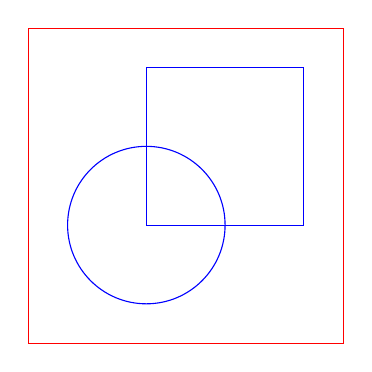
\begin{tikzpicture}[blue,baseline=0pt]
\draw [red,use as bounding box] (-1.5,-1.5) rectangle (2.5,2.5);
\draw (0,0) rectangle(2,2); 
 \draw (0,0) circle (1);
\end{tikzpicture}
\TFRGB{texte après}{text after} 
&  
\parbox[c]{10cm}{
\TFRGB{texte avant}{text before} \\
\BS{begin}\AC{tikzpicture}[blue,\RDD{baseline}=0pt] \\
\BS{draw} [red,\RDD{use as bounding box}] (-1.5,-1.5) rectangle (2.5,2.5);\\
\BS{draw} (0,0) rectangle(2,2);  \\
\BS{draw} (0,0) circle (1); \\
\BS{end}\AC{tikzpicture} \\
\TFRGB{texte après}{text after} \\
}
\\ \hline 
\end{tabular}

\bigskip

\begin{tabular}{|l|l|} \hline 
\TFRGB{texte avant}{text before} 
\begin{tikzpicture}[blue,baseline=0pt]
\useasboundingbox  (-1.5,-1.5) rectangle (2.5,2.5);
\draw (0,0) rectangle(2,2); 
 \draw (0,0) circle (1);
\end{tikzpicture}
\TFRGB{texte après}{text after} 
&  
\parbox[c]{10cm}{
\TFRGB{texte avant}{text before} \\
\BS{begin}\AC{tikzpicture}[blue,baseline=0pt] \\
\BSS{useasboundingbox}  (-1.5,-1.5) rectangle (2.5,2.5);\\
\BS{draw} (0,0) rectangle(2,2);  \\
\BS{draw} (0,0) circle (1); \\
\BS{end}\AC{tikzpicture} \\
\TFRGB{texte après}{text after} \\
}
\\ \hline 
\end{tabular}

\bigskip

\begin{tabular}{|c|c|} \hline  
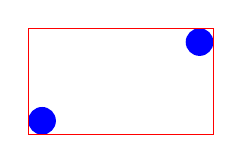
\begin{tikzpicture}[blue,baseline=0pt]
\fill (0,0) circle (5pt);
\fill (2,1) circle (5pt);
\draw[red] (current bounding box.south west) rectangle
(current bounding box.north east);
\end{tikzpicture}
&  
\parbox[c]{14cm}{
\BS{begin}\AC{tikzpicture}[blue] \\
\BS{fill} (0,0) circle (5pt); \\
\BS{fill}  (2,1) circle (5pt);\\
\BS{draw}[red] (\RDD{current bounding box.south west}) rectangle
(\RDD{current bounding box.north east});\\
\BS{end}\AC{tikzpicture}
}
\\ \hline 
\end{tabular}
\newpage
\SbSSCT{Coupure de l'image}{Clipping the picture}
	
\begin{center}
\RRR{15-9}
\end{center}

\begin{tabular}{|c|c|} \hline  
\tikzpicture[red]
\draw[help lines] (-2,-2) grid (2,2);
\draw[blue] (-1,-1) --(0,2) -- (1,-1) -- cycle;
\draw (0,0) circle (.5);
\draw (0,0) circle (1);
\draw (0,0) circle (1.5);
\endtikzpicture
&  
\tikzpicture[red]
\clip (-1,-1) --(0,2) -- (1,-1) -- cycle;
\draw[help lines] (-2,-2) grid (2,2);
\draw[blue] (-1,-1) --(0,2) -- (1,-1) -- cycle;
\draw (0,0) circle (.5);
\draw (0,0) circle (1);
\draw (0,0) circle (1.5);
\endtikzpicture
\\ \hline  
\TFRGB{sans coupure}{no clipping}
&  
\BSS{clip} (-1,-1) - -(0,2) - - (1,-1) - - cycle;
\\ \hline 
\end{tabular} 



\SbSSCT{Rognage partiel}{ Partial clipping}

\noindent

\begin{tabular}{|c|c|} \hline   
\tikzpicture[red,scale=.7,baseline=0pt]
\draw[help lines] (-2,-2) grid (2,2);
\draw[blue] (-1.1,-0.2) rectangle (2,1.5);
\draw (0,0) circle (1.5);
\clip (-1.1,-0.2) rectangle (2,1.5);
\draw (0,0) circle (.5);
\draw (0,0) circle (1);
\endtikzpicture
& 
\parbox{8cm}{ 
\BS{tikzpicture}[red,scale=.7] \\
\BS{draw}[help lines] (-2,-2) grid (2,2); \\
\BS{draw}[blue] (-1.1,-0.2) rectangle (2,1.5); \\
\BS{draw} (0,0) circle (1.5); \\
\BSS{clip} (-1.1,-0.2) rectangle (2,1.5); \\
\BS{draw} (0,0) circle (.5); \\
\BS{draw} (0,0) circle (1); \\
\BS{endtikzpicture}} 
\\ \hline 
\end{tabular}

%\subsubsection{Changement d'échelle}
\SbSbSSCT{Changement d'échelle}{Scaling}

\noindent

\begin{tabular}{|c|c|} \hline  
\tikzpicture[blue]
\draw[help lines] (-2,-2) grid (2,2);
\draw (0,0) circle (.5);
\draw (0,0) circle (1);
\draw (0,0) circle (1.5);
\endtikzpicture
&  
\tikzpicture[blue,scale=.5]
\draw[help lines] (-2,-2) grid (2,2);
\draw (0,0) circle (.5);
\draw (0,0) circle (1);
\draw (0,0) circle (1.5);
\endtikzpicture
\\ \hline  
\TFRGB{Taille normale}{Normal size}
&  
\BS{tikzpicture}[blue,\RDD{scale}=.5]
\\ \hline 
\end{tabular} 

